% Created by tikzDevice version 0.12.3.2 on 2022-02-18 15:29:53
% !TEX encoding = UTF-8 Unicode
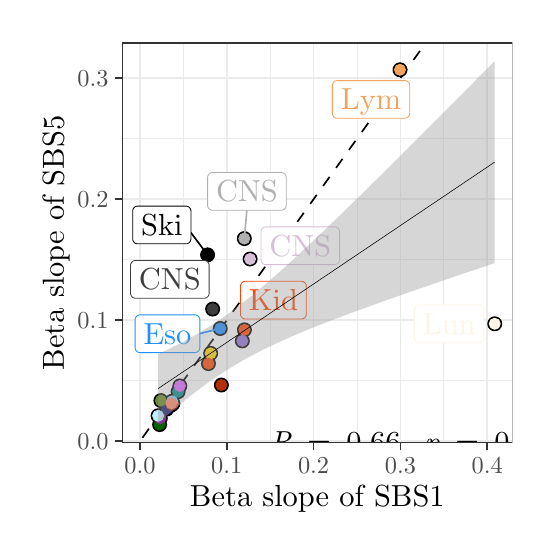
\begin{tikzpicture}[x=1pt,y=1pt]
\definecolor{fillColor}{RGB}{255,255,255}
\path[use as bounding box,fill=fillColor,fill opacity=0.00] (0,0) rectangle (180.67,180.67);
\begin{scope}
\path[clip] (  0.00,  0.00) rectangle (180.67,180.67);
\definecolor{drawColor}{RGB}{255,255,255}
\definecolor{fillColor}{RGB}{255,255,255}

\path[draw=drawColor,line width= 0.6pt,line join=round,line cap=round,fill=fillColor] (  0.00,  0.00) rectangle (180.68,180.68);
\end{scope}
\begin{scope}
\path[clip] ( 34.16, 30.69) rectangle (175.17,175.17);
\definecolor{fillColor}{RGB}{255,255,255}

\path[fill=fillColor] ( 34.16, 30.69) rectangle (175.17,175.17);
\definecolor{drawColor}{gray}{0.92}

\path[draw=drawColor,line width= 0.3pt,line join=round] ( 34.16, 53.08) --
	(175.17, 53.08);

\path[draw=drawColor,line width= 0.3pt,line join=round] ( 34.16, 96.81) --
	(175.17, 96.81);

\path[draw=drawColor,line width= 0.3pt,line join=round] ( 34.16,140.54) --
	(175.17,140.54);

\path[draw=drawColor,line width= 0.3pt,line join=round] ( 56.25, 30.69) --
	( 56.25,175.17);

\path[draw=drawColor,line width= 0.3pt,line join=round] ( 87.62, 30.69) --
	( 87.62,175.17);

\path[draw=drawColor,line width= 0.3pt,line join=round] (118.99, 30.69) --
	(118.99,175.17);

\path[draw=drawColor,line width= 0.3pt,line join=round] (150.36, 30.69) --
	(150.36,175.17);

\path[draw=drawColor,line width= 0.6pt,line join=round] ( 34.16, 31.21) --
	(175.17, 31.21);

\path[draw=drawColor,line width= 0.6pt,line join=round] ( 34.16, 74.94) --
	(175.17, 74.94);

\path[draw=drawColor,line width= 0.6pt,line join=round] ( 34.16,118.68) --
	(175.17,118.68);

\path[draw=drawColor,line width= 0.6pt,line join=round] ( 34.16,162.41) --
	(175.17,162.41);

\path[draw=drawColor,line width= 0.6pt,line join=round] ( 40.57, 30.69) --
	( 40.57,175.17);

\path[draw=drawColor,line width= 0.6pt,line join=round] ( 71.94, 30.69) --
	( 71.94,175.17);

\path[draw=drawColor,line width= 0.6pt,line join=round] (103.31, 30.69) --
	(103.31,175.17);

\path[draw=drawColor,line width= 0.6pt,line join=round] (134.68, 30.69) --
	(134.68,175.17);

\path[draw=drawColor,line width= 0.6pt,line join=round] (166.05, 30.69) --
	(166.05,175.17);
\definecolor{drawColor}{RGB}{0,0,0}

\path[draw=drawColor,line width= 0.6pt,dash pattern=on 4pt off 4pt ,line join=round] ( 18.18,  0.00) -- (147.78,180.67);
\definecolor{fillColor}{RGB}{0,0,0}

\path[draw=drawColor,line width= 0.4pt,line join=round,line cap=round,fill=fillColor] ( 66.12, 62.98) circle (  2.50);

\path[draw=drawColor,line width= 0.4pt,line join=round,line cap=round,fill=fillColor] ( 52.47, 44.81) circle (  2.50);

\path[draw=drawColor,line width= 0.4pt,line join=round,line cap=round,fill=fillColor] ( 66.84, 78.98) circle (  2.50);

\path[draw=drawColor,line width= 0.4pt,line join=round,line cap=round,fill=fillColor] ( 80.37, 97.08) circle (  2.50);

\path[draw=drawColor,line width= 0.4pt,line join=round,line cap=round,fill=fillColor] ( 78.28,104.46) circle (  2.50);

\path[draw=drawColor,line width= 0.4pt,line join=round,line cap=round,fill=fillColor] ( 50.24, 42.86) circle (  2.50);

\path[draw=drawColor,line width= 0.4pt,line join=round,line cap=round,fill=fillColor] ( 69.57, 71.97) circle (  2.50);

\path[draw=drawColor,line width= 0.4pt,line join=round,line cap=round,fill=fillColor] ( 51.99, 44.35) circle (  2.50);

\path[draw=drawColor,line width= 0.4pt,line join=round,line cap=round,fill=fillColor] ( 70.00, 51.54) circle (  2.50);

\path[draw=drawColor,line width= 0.4pt,line join=round,line cap=round,fill=fillColor] ( 78.32, 71.48) circle (  2.50);

\path[draw=drawColor,line width= 0.4pt,line join=round,line cap=round,fill=fillColor] ( 65.32, 59.29) circle (  2.50);

\path[draw=drawColor,line width= 0.4pt,line join=round,line cap=round,fill=fillColor] ( 47.67, 37.25) circle (  2.50);

\path[draw=drawColor,line width= 0.4pt,line join=round,line cap=round,fill=fillColor] (168.77, 73.67) circle (  2.50);

\path[draw=drawColor,line width= 0.4pt,line join=round,line cap=round,fill=fillColor] ( 48.14, 45.91) circle (  2.50);

\path[draw=drawColor,line width= 0.4pt,line join=round,line cap=round,fill=fillColor] (134.53,165.45) circle (  2.50);

\path[draw=drawColor,line width= 0.4pt,line join=round,line cap=round,fill=fillColor] ( 54.35, 49.14) circle (  2.50);

\path[draw=drawColor,line width= 0.4pt,line join=round,line cap=round,fill=fillColor] ( 47.92, 39.53) circle (  2.50);

\path[draw=drawColor,line width= 0.4pt,line join=round,line cap=round,fill=fillColor] ( 54.98, 51.21) circle (  2.50);

\path[draw=drawColor,line width= 0.4pt,line join=round,line cap=round,fill=fillColor] ( 52.18, 45.68) circle (  2.50);

\path[draw=drawColor,line width= 0.4pt,line join=round,line cap=round,fill=fillColor] ( 65.01, 98.57) circle (  2.50);

\path[draw=drawColor,line width= 0.4pt,line join=round,line cap=round,fill=fillColor] ( 47.12, 40.43) circle (  2.50);

\path[draw=drawColor,line width= 0.4pt,line join=round,line cap=round,fill=fillColor] ( 77.56, 67.49) circle (  2.50);

\path[draw=drawColor,line width= 0.4pt,line join=round,line cap=round,fill=fillColor] ( 51.95, 44.90) circle (  2.50);
\definecolor{drawColor}{RGB}{255,215,0}
\definecolor{fillColor}{RGB}{255,215,0}

\path[draw=drawColor,line width= 0.4pt,line join=round,line cap=round,fill=fillColor] ( 66.12, 62.98) circle (  1.96);
\definecolor{drawColor}{RGB}{205,96,144}
\definecolor{fillColor}{RGB}{205,96,144}

\path[draw=drawColor,line width= 0.4pt,line join=round,line cap=round,fill=fillColor] ( 52.47, 44.81) circle (  1.96);
\definecolor{drawColor}{gray}{0.24}
\definecolor{fillColor}{gray}{0.24}

\path[draw=drawColor,line width= 0.4pt,line join=round,line cap=round,fill=fillColor] ( 66.84, 78.98) circle (  1.96);
\definecolor{drawColor}{RGB}{216,191,216}
\definecolor{fillColor}{RGB}{216,191,216}

\path[draw=drawColor,line width= 0.4pt,line join=round,line cap=round,fill=fillColor] ( 80.37, 97.08) circle (  1.96);
\definecolor{drawColor}{gray}{0.69}
\definecolor{fillColor}{gray}{0.69}

\path[draw=drawColor,line width= 0.4pt,line join=round,line cap=round,fill=fillColor] ( 78.28,104.46) circle (  1.96);
\definecolor{drawColor}{RGB}{25,25,112}
\definecolor{fillColor}{RGB}{25,25,112}

\path[draw=drawColor,line width= 0.4pt,line join=round,line cap=round,fill=fillColor] ( 50.24, 42.86) circle (  1.96);
\definecolor{drawColor}{RGB}{30,144,255}
\definecolor{fillColor}{RGB}{30,144,255}

\path[draw=drawColor,line width= 0.4pt,line join=round,line cap=round,fill=fillColor] ( 69.57, 71.97) circle (  1.96);
\definecolor{drawColor}{RGB}{139,35,35}
\definecolor{fillColor}{RGB}{139,35,35}

\path[draw=drawColor,line width= 0.4pt,line join=round,line cap=round,fill=fillColor] ( 51.99, 44.35) circle (  1.96);
\definecolor{drawColor}{RGB}{179,47,11}
\definecolor{fillColor}{RGB}{179,47,11}

\path[draw=drawColor,line width= 0.4pt,line join=round,line cap=round,fill=fillColor] ( 70.00, 51.54) circle (  1.96);
\definecolor{drawColor}{RGB}{255,69,0}
\definecolor{fillColor}{RGB}{255,69,0}

\path[draw=drawColor,line width= 0.4pt,line join=round,line cap=round,fill=fillColor] ( 78.32, 71.48) circle (  1.96);

\path[draw=drawColor,line width= 0.4pt,line join=round,line cap=round,fill=fillColor] ( 65.32, 59.29) circle (  1.96);
\definecolor{drawColor}{RGB}{0,100,0}
\definecolor{fillColor}{RGB}{0,100,0}

\path[draw=drawColor,line width= 0.4pt,line join=round,line cap=round,fill=fillColor] ( 47.67, 37.25) circle (  1.96);
\definecolor{drawColor}{RGB}{253,245,230}
\definecolor{fillColor}{RGB}{253,245,230}

\path[draw=drawColor,line width= 0.4pt,line join=round,line cap=round,fill=fillColor] (168.77, 73.67) circle (  1.96);
\definecolor{drawColor}{RGB}{105,139,34}
\definecolor{fillColor}{RGB}{105,139,34}

\path[draw=drawColor,line width= 0.4pt,line join=round,line cap=round,fill=fillColor] ( 48.14, 45.91) circle (  1.96);
\definecolor{drawColor}{RGB}{244,163,93}
\definecolor{fillColor}{RGB}{244,163,93}

\path[draw=drawColor,line width= 0.4pt,line join=round,line cap=round,fill=fillColor] (134.53,165.45) circle (  1.96);
\definecolor{drawColor}{RGB}{0,139,139}
\definecolor{fillColor}{RGB}{0,139,139}

\path[draw=drawColor,line width= 0.4pt,line join=round,line cap=round,fill=fillColor] ( 54.35, 49.14) circle (  1.96);
\definecolor{drawColor}{RGB}{122,55,139}
\definecolor{fillColor}{RGB}{122,55,139}

\path[draw=drawColor,line width= 0.4pt,line join=round,line cap=round,fill=fillColor] ( 47.92, 39.53) circle (  1.96);
\definecolor{drawColor}{RGB}{224,102,255}
\definecolor{fillColor}{RGB}{224,102,255}

\path[draw=drawColor,line width= 0.4pt,line join=round,line cap=round,fill=fillColor] ( 54.98, 51.21) circle (  1.96);
\definecolor{drawColor}{RGB}{135,206,250}
\definecolor{fillColor}{RGB}{135,206,250}

\path[draw=drawColor,line width= 0.4pt,line join=round,line cap=round,fill=fillColor] ( 52.18, 45.68) circle (  1.96);
\definecolor{drawColor}{RGB}{0,0,0}
\definecolor{fillColor}{RGB}{0,0,0}

\path[draw=drawColor,line width= 0.4pt,line join=round,line cap=round,fill=fillColor] ( 65.01, 98.57) circle (  1.96);
\definecolor{drawColor}{RGB}{191,239,255}
\definecolor{fillColor}{RGB}{191,239,255}

\path[draw=drawColor,line width= 0.4pt,line join=round,line cap=round,fill=fillColor] ( 47.12, 40.43) circle (  1.96);
\definecolor{drawColor}{RGB}{147,112,219}
\definecolor{fillColor}{RGB}{147,112,219}

\path[draw=drawColor,line width= 0.4pt,line join=round,line cap=round,fill=fillColor] ( 77.56, 67.49) circle (  1.96);
\definecolor{drawColor}{RGB}{255,140,105}
\definecolor{fillColor}{RGB}{255,140,105}

\path[draw=drawColor,line width= 0.4pt,line join=round,line cap=round,fill=fillColor] ( 51.95, 44.90) circle (  1.96);
\end{scope}
\begin{scope}
\path[clip] ( 34.16, 30.69) rectangle (175.17,175.17);
\definecolor{drawColor}{gray}{0.69}

\path[draw=drawColor,line width= 0.6pt,line join=round,line cap=round] ( 79.21,114.68) -- ( 78.36,105.39);
\definecolor{drawColor}{RGB}{30,144,255}

\path[draw=drawColor,line width= 0.6pt,line join=round,line cap=round] ( 62.22, 70.13) -- ( 68.69, 71.75);
\definecolor{drawColor}{RGB}{0,0,0}

\path[draw=drawColor,line width= 0.6pt,line join=round,line cap=round] ( 58.99,106.59) -- ( 64.45, 99.31);
\definecolor{drawColor}{gray}{0.24}
\definecolor{fillColor}{RGB}{255,255,255}

\path[draw=drawColor,line width= 0.3pt,line join=round,line cap=round,fill=fillColor] ( 38.97, 82.91) --
	( 63.76, 82.91) --
	( 63.69, 82.91) --
	( 63.98, 82.92) --
	( 64.27, 82.98) --
	( 64.54, 83.08) --
	( 64.79, 83.23) --
	( 65.02, 83.41) --
	( 65.21, 83.63) --
	( 65.36, 83.88) --
	( 65.48, 84.14) --
	( 65.55, 84.43) --
	( 65.57, 84.72) --
	( 65.57, 84.72) --
	( 65.57, 94.73) --
	( 65.57, 94.73) --
	( 65.55, 95.02) --
	( 65.48, 95.30) --
	( 65.36, 95.57) --
	( 65.21, 95.81) --
	( 65.02, 96.03) --
	( 64.79, 96.22) --
	( 64.54, 96.36) --
	( 64.27, 96.46) --
	( 63.98, 96.52) --
	( 63.76, 96.54) --
	( 38.97, 96.54) --
	( 39.19, 96.52) --
	( 38.90, 96.53) --
	( 38.61, 96.50) --
	( 38.33, 96.42) --
	( 38.07, 96.29) --
	( 37.83, 96.13) --
	( 37.62, 95.93) --
	( 37.45, 95.69) --
	( 37.31, 95.44) --
	( 37.22, 95.16) --
	( 37.17, 94.87) --
	( 37.17, 94.73) --
	( 37.17, 84.72) --
	( 37.17, 84.86) --
	( 37.17, 84.57) --
	( 37.22, 84.28) --
	( 37.31, 84.01) --
	( 37.45, 83.75) --
	( 37.62, 83.52) --
	( 37.83, 83.32) --
	( 38.07, 83.15) --
	( 38.33, 83.03) --
	( 38.61, 82.95) --
	( 38.90, 82.91) --
	cycle;
\end{scope}
\begin{scope}
\path[clip] ( 34.16, 30.69) rectangle (175.17,175.17);
\definecolor{drawColor}{gray}{0.24}

\node[text=drawColor,anchor=base,inner sep=0pt, outer sep=0pt, scale=  1.10] at ( 51.37, 85.92) {CNS};
\definecolor{drawColor}{RGB}{216,191,216}
\definecolor{fillColor}{RGB}{255,255,255}

\path[draw=drawColor,line width= 0.3pt,line join=round,line cap=round,fill=fillColor] ( 86.11, 95.06) --
	(110.90, 95.06) --
	(110.83, 95.06) --
	(111.12, 95.07) --
	(111.40, 95.13) --
	(111.67, 95.23) --
	(111.93, 95.38) --
	(112.15, 95.56) --
	(112.34, 95.78) --
	(112.50, 96.03) --
	(112.61, 96.29) --
	(112.68, 96.58) --
	(112.71, 96.87) --
	(112.71, 96.87) --
	(112.71,106.88) --
	(112.71,106.88) --
	(112.68,107.17) --
	(112.61,107.45) --
	(112.50,107.72) --
	(112.34,107.96) --
	(112.15,108.18) --
	(111.93,108.37) --
	(111.67,108.51) --
	(111.40,108.61) --
	(111.12,108.67) --
	(110.90,108.69) --
	( 86.11,108.69) --
	( 86.33,108.67) --
	( 86.04,108.68) --
	( 85.75,108.65) --
	( 85.47,108.57) --
	( 85.21,108.44) --
	( 84.97,108.28) --
	( 84.76,108.08) --
	( 84.58,107.84) --
	( 84.45,107.59) --
	( 84.36,107.31) --
	( 84.31,107.02) --
	( 84.30,106.88) --
	( 84.30, 96.87) --
	( 84.31, 97.01) --
	( 84.31, 96.72) --
	( 84.36, 96.43) --
	( 84.45, 96.16) --
	( 84.58, 95.90) --
	( 84.76, 95.67) --
	( 84.97, 95.47) --
	( 85.21, 95.30) --
	( 85.47, 95.18) --
	( 85.75, 95.10) --
	( 86.04, 95.06) --
	cycle;
\end{scope}
\begin{scope}
\path[clip] ( 34.16, 30.69) rectangle (175.17,175.17);
\definecolor{drawColor}{RGB}{216,191,216}

\node[text=drawColor,anchor=base,inner sep=0pt, outer sep=0pt, scale=  1.10] at ( 98.50, 98.07) {CNS};
\definecolor{drawColor}{gray}{0.69}
\definecolor{fillColor}{RGB}{255,255,255}

\path[draw=drawColor,line width= 0.3pt,line join=round,line cap=round,fill=fillColor] ( 66.82,114.68) --
	( 91.61,114.68) --
	( 91.54,114.68) --
	( 91.83,114.70) --
	( 92.11,114.75) --
	( 92.38,114.86) --
	( 92.64,115.00) --
	( 92.86,115.19) --
	( 93.05,115.40) --
	( 93.21,115.65) --
	( 93.32,115.92) --
	( 93.39,116.20) --
	( 93.42,116.49) --
	( 93.42,116.49) --
	( 93.42,126.50) --
	( 93.42,126.50) --
	( 93.39,126.79) --
	( 93.32,127.07) --
	( 93.21,127.34) --
	( 93.05,127.59) --
	( 92.86,127.80) --
	( 92.64,127.99) --
	( 92.38,128.13) --
	( 92.11,128.24) --
	( 91.83,128.29) --
	( 91.61,128.31) --
	( 66.82,128.31) --
	( 67.04,128.29) --
	( 66.75,128.31) --
	( 66.46,128.27) --
	( 66.18,128.19) --
	( 65.92,128.07) --
	( 65.68,127.90) --
	( 65.47,127.70) --
	( 65.29,127.47) --
	( 65.16,127.21) --
	( 65.07,126.93) --
	( 65.02,126.65) --
	( 65.01,126.50) --
	( 65.01,116.49) --
	( 65.02,116.63) --
	( 65.02,116.34) --
	( 65.07,116.06) --
	( 65.16,115.78) --
	( 65.29,115.52) --
	( 65.47,115.29) --
	( 65.68,115.09) --
	( 65.92,114.92) --
	( 66.18,114.80) --
	( 66.46,114.72) --
	( 66.75,114.68) --
	cycle;
\end{scope}
\begin{scope}
\path[clip] ( 34.16, 30.69) rectangle (175.17,175.17);
\definecolor{drawColor}{gray}{0.69}

\node[text=drawColor,anchor=base,inner sep=0pt, outer sep=0pt, scale=  1.10] at ( 79.21,117.69) {CNS};
\definecolor{drawColor}{RGB}{30,144,255}
\definecolor{fillColor}{RGB}{255,255,255}

\path[draw=drawColor,line width= 0.3pt,line join=round,line cap=round,fill=fillColor] ( 40.62, 63.26) --
	( 60.42, 63.26) --
	( 60.34, 63.27) --
	( 60.63, 63.28) --
	( 60.92, 63.34) --
	( 61.19, 63.44) --
	( 61.44, 63.58) --
	( 61.67, 63.77) --
	( 61.86, 63.99) --
	( 62.02, 64.23) --
	( 62.13, 64.50) --
	( 62.20, 64.78) --
	( 62.22, 65.07) --
	( 62.22, 65.07) --
	( 62.22, 75.08) --
	( 62.22, 75.08) --
	( 62.20, 75.37) --
	( 62.13, 75.66) --
	( 62.02, 75.92) --
	( 61.86, 76.17) --
	( 61.67, 76.39) --
	( 61.44, 76.57) --
	( 61.19, 76.72) --
	( 60.92, 76.82) --
	( 60.63, 76.88) --
	( 60.42, 76.89) --
	( 40.62, 76.89) --
	( 40.84, 76.88) --
	( 40.55, 76.89) --
	( 40.26, 76.85) --
	( 39.98, 76.77) --
	( 39.72, 76.65) --
	( 39.48, 76.48) --
	( 39.27, 76.28) --
	( 39.10, 76.05) --
	( 38.96, 75.79) --
	( 38.87, 75.52) --
	( 38.82, 75.23) --
	( 38.82, 75.08) --
	( 38.82, 65.07) --
	( 38.82, 65.22) --
	( 38.82, 64.93) --
	( 38.87, 64.64) --
	( 38.96, 64.36) --
	( 39.10, 64.11) --
	( 39.27, 63.87) --
	( 39.48, 63.67) --
	( 39.72, 63.51) --
	( 39.98, 63.38) --
	( 40.26, 63.30) --
	( 40.55, 63.27) --
	cycle;
\end{scope}
\begin{scope}
\path[clip] ( 34.16, 30.69) rectangle (175.17,175.17);
\definecolor{drawColor}{RGB}{30,144,255}

\node[text=drawColor,anchor=base,inner sep=0pt, outer sep=0pt, scale=  1.10] at ( 50.52, 66.28) {Eso};
\definecolor{drawColor}{RGB}{255,69,0}
\definecolor{fillColor}{RGB}{255,255,255}

\path[draw=drawColor,line width= 0.3pt,line join=round,line cap=round,fill=fillColor] ( 78.69, 75.39) --
	( 98.88, 75.39) --
	( 98.81, 75.40) --
	( 99.10, 75.41) --
	( 99.39, 75.47) --
	( 99.66, 75.57) --
	( 99.91, 75.71) --
	(100.13, 75.90) --
	(100.33, 76.12) --
	(100.48, 76.36) --
	(100.60, 76.63) --
	(100.67, 76.91) --
	(100.69, 77.20) --
	(100.69, 77.20) --
	(100.69, 87.21) --
	(100.69, 87.21) --
	(100.67, 87.50) --
	(100.60, 87.79) --
	(100.48, 88.05) --
	(100.33, 88.30) --
	(100.13, 88.52) --
	( 99.91, 88.70) --
	( 99.66, 88.85) --
	( 99.39, 88.95) --
	( 99.10, 89.01) --
	( 98.88, 89.02) --
	( 78.69, 89.02) --
	( 78.91, 89.01) --
	( 78.62, 89.02) --
	( 78.33, 88.98) --
	( 78.05, 88.90) --
	( 77.79, 88.78) --
	( 77.55, 88.61) --
	( 77.34, 88.41) --
	( 77.16, 88.18) --
	( 77.03, 87.92) --
	( 76.94, 87.65) --
	( 76.89, 87.36) --
	( 76.88, 87.21) --
	( 76.88, 77.20) --
	( 76.89, 77.35) --
	( 76.89, 77.06) --
	( 76.94, 76.77) --
	( 77.03, 76.49) --
	( 77.16, 76.24) --
	( 77.34, 76.00) --
	( 77.55, 75.80) --
	( 77.79, 75.64) --
	( 78.05, 75.51) --
	( 78.33, 75.43) --
	( 78.62, 75.40) --
	cycle;
\end{scope}
\begin{scope}
\path[clip] ( 34.16, 30.69) rectangle (175.17,175.17);
\definecolor{drawColor}{RGB}{255,69,0}

\node[text=drawColor,anchor=base,inner sep=0pt, outer sep=0pt, scale=  1.10] at ( 88.79, 78.41) {Kid};
\definecolor{drawColor}{RGB}{253,245,230}
\definecolor{fillColor}{RGB}{255,255,255}

\path[draw=drawColor,line width= 0.3pt,line join=round,line cap=round,fill=fillColor] (141.52, 66.84) --
	(163.09, 66.84) --
	(163.02, 66.84) --
	(163.31, 66.85) --
	(163.59, 66.91) --
	(163.86, 67.01) --
	(164.12, 67.16) --
	(164.34, 67.34) --
	(164.53, 67.56) --
	(164.69, 67.81) --
	(164.80, 68.07) --
	(164.87, 68.36) --
	(164.90, 68.65) --
	(164.90, 68.65) --
	(164.90, 78.66) --
	(164.90, 78.66) --
	(164.87, 78.95) --
	(164.80, 79.23) --
	(164.69, 79.50) --
	(164.53, 79.74) --
	(164.34, 79.96) --
	(164.12, 80.14) --
	(163.86, 80.29) --
	(163.59, 80.39) --
	(163.31, 80.45) --
	(163.09, 80.46) --
	(141.52, 80.46) --
	(141.74, 80.45) --
	(141.45, 80.46) --
	(141.16, 80.43) --
	(140.88, 80.35) --
	(140.61, 80.22) --
	(140.38, 80.06) --
	(140.17, 79.86) --
	(139.99, 79.62) --
	(139.86, 79.37) --
	(139.76, 79.09) --
	(139.72, 78.80) --
	(139.71, 78.66) --
	(139.71, 68.65) --
	(139.72, 68.79) --
	(139.72, 68.50) --
	(139.76, 68.21) --
	(139.86, 67.94) --
	(139.99, 67.68) --
	(140.17, 67.45) --
	(140.38, 67.25) --
	(140.61, 67.08) --
	(140.88, 66.96) --
	(141.16, 66.88) --
	(141.45, 66.84) --
	cycle;
\end{scope}
\begin{scope}
\path[clip] ( 34.16, 30.69) rectangle (175.17,175.17);
\definecolor{drawColor}{RGB}{253,245,230}

\node[text=drawColor,anchor=base,inner sep=0pt, outer sep=0pt, scale=  1.10] at (152.30, 69.85) {Lun};
\definecolor{drawColor}{RGB}{244,163,93}
\definecolor{fillColor}{RGB}{255,255,255}

\path[draw=drawColor,line width= 0.3pt,line join=round,line cap=round,fill=fillColor] (111.91,147.92) --
	(136.24,147.92) --
	(136.16,147.92) --
	(136.45,147.93) --
	(136.74,147.99) --
	(137.01,148.09) --
	(137.26,148.24) --
	(137.49,148.42) --
	(137.68,148.64) --
	(137.84,148.88) --
	(137.95,149.15) --
	(138.02,149.43) --
	(138.04,149.72) --
	(138.04,149.72) --
	(138.04,159.74) --
	(138.04,159.74) --
	(138.02,160.03) --
	(137.95,160.31) --
	(137.84,160.58) --
	(137.68,160.82) --
	(137.49,161.04) --
	(137.26,161.22) --
	(137.01,161.37) --
	(136.74,161.47) --
	(136.45,161.53) --
	(136.24,161.54) --
	(111.91,161.54) --
	(112.12,161.53) --
	(111.83,161.54) --
	(111.54,161.51) --
	(111.26,161.43) --
	(111.00,161.30) --
	(110.76,161.14) --
	(110.55,160.94) --
	(110.38,160.70) --
	(110.24,160.45) --
	(110.15,160.17) --
	(110.10,159.88) --
	(110.10,159.74) --
	(110.10,149.72) --
	(110.10,149.87) --
	(110.10,149.58) --
	(110.15,149.29) --
	(110.24,149.02) --
	(110.38,148.76) --
	(110.55,148.53) --
	(110.76,148.32) --
	(111.00,148.16) --
	(111.26,148.04) --
	(111.54,147.95) --
	(111.83,147.92) --
	cycle;
\end{scope}
\begin{scope}
\path[clip] ( 34.16, 30.69) rectangle (175.17,175.17);
\definecolor{drawColor}{RGB}{244,163,93}

\node[text=drawColor,anchor=base,inner sep=0pt, outer sep=0pt, scale=  1.10] at (124.07,150.93) {Lym};
\definecolor{drawColor}{RGB}{0,0,0}
\definecolor{fillColor}{RGB}{255,255,255}

\path[draw=drawColor,line width= 0.3pt,line join=round,line cap=round,fill=fillColor] ( 39.75,102.56) --
	( 57.18,102.56) --
	( 57.11,102.57) --
	( 57.40,102.58) --
	( 57.69,102.64) --
	( 57.96,102.74) --
	( 58.21,102.88) --
	( 58.44,103.07) --
	( 58.63,103.29) --
	( 58.78,103.53) --
	( 58.90,103.80) --
	( 58.97,104.08) --
	( 58.99,104.37) --
	( 58.99,104.37) --
	( 58.99,114.38) --
	( 58.99,114.38) --
	( 58.97,114.67) --
	( 58.90,114.96) --
	( 58.78,115.22) --
	( 58.63,115.47) --
	( 58.44,115.69) --
	( 58.21,115.87) --
	( 57.96,116.02) --
	( 57.69,116.12) --
	( 57.40,116.18) --
	( 57.18,116.19) --
	( 39.75,116.19) --
	( 39.97,116.18) --
	( 39.68,116.19) --
	( 39.39,116.15) --
	( 39.11,116.07) --
	( 38.85,115.95) --
	( 38.61,115.78) --
	( 38.40,115.58) --
	( 38.22,115.35) --
	( 38.09,115.09) --
	( 38.00,114.82) --
	( 37.95,114.53) --
	( 37.95,114.38) --
	( 37.95,104.37) --
	( 37.95,104.52) --
	( 37.95,104.23) --
	( 38.00,103.94) --
	( 38.09,103.66) --
	( 38.22,103.41) --
	( 38.40,103.17) --
	( 38.61,102.97) --
	( 38.85,102.81) --
	( 39.11,102.68) --
	( 39.39,102.60) --
	( 39.68,102.57) --
	cycle;
\end{scope}
\begin{scope}
\path[clip] ( 34.16, 30.69) rectangle (175.17,175.17);
\definecolor{drawColor}{RGB}{0,0,0}

\node[text=drawColor,anchor=base,inner sep=0pt, outer sep=0pt, scale=  1.10] at ( 48.47,105.58) {Ski};
\definecolor{fillColor}{RGB}{153,153,153}

\path[fill=fillColor,fill opacity=0.40] ( 47.12, 62.71) --
	( 48.66, 63.42) --
	( 50.20, 64.15) --
	( 51.74, 64.90) --
	( 53.28, 65.67) --
	( 54.82, 66.46) --
	( 56.36, 67.27) --
	( 57.90, 68.10) --
	( 59.44, 68.96) --
	( 60.98, 69.84) --
	( 62.52, 70.75) --
	( 64.06, 71.68) --
	( 65.60, 72.65) --
	( 67.14, 73.64) --
	( 68.68, 74.66) --
	( 70.22, 75.71) --
	( 71.76, 76.79) --
	( 73.30, 77.90) --
	( 74.84, 79.04) --
	( 76.38, 80.20) --
	( 77.92, 81.39) --
	( 79.46, 82.61) --
	( 81.00, 83.85) --
	( 82.54, 85.11) --
	( 84.08, 86.40) --
	( 85.62, 87.70) --
	( 87.16, 89.03) --
	( 88.70, 90.37) --
	( 90.24, 91.72) --
	( 91.78, 93.10) --
	( 93.32, 94.48) --
	( 94.86, 95.88) --
	( 96.39, 97.29) --
	( 97.93, 98.71) --
	( 99.47,100.14) --
	(101.01,101.58) --
	(102.55,103.02) --
	(104.09,104.48) --
	(105.63,105.94) --
	(107.17,107.41) --
	(108.71,108.89) --
	(110.25,110.37) --
	(111.79,111.85) --
	(113.33,113.34) --
	(114.87,114.84) --
	(116.41,116.34) --
	(117.95,117.84) --
	(119.49,119.35) --
	(121.03,120.86) --
	(122.57,122.37) --
	(124.11,123.89) --
	(125.65,125.41) --
	(127.19,126.93) --
	(128.73,128.45) --
	(130.27,129.98) --
	(131.81,131.51) --
	(133.35,133.04) --
	(134.89,134.57) --
	(136.43,136.11) --
	(137.97,137.64) --
	(139.51,139.18) --
	(141.05,140.72) --
	(142.59,142.26) --
	(144.13,143.80) --
	(145.67,145.34) --
	(147.21,146.89) --
	(148.75,148.43) --
	(150.29,149.98) --
	(151.83,151.53) --
	(153.37,153.08) --
	(154.91,154.63) --
	(156.45,156.18) --
	(157.99,157.73) --
	(159.53,159.28) --
	(161.07,160.83) --
	(162.61,162.39) --
	(164.15,163.94) --
	(165.69,165.50) --
	(167.23,167.05) --
	(168.77,168.61) --
	(168.77, 95.61) --
	(167.23, 95.09) --
	(165.69, 94.58) --
	(164.15, 94.06) --
	(162.61, 93.54) --
	(161.07, 93.02) --
	(159.53, 92.50) --
	(157.99, 91.98) --
	(156.45, 91.46) --
	(154.91, 90.93) --
	(153.37, 90.41) --
	(151.83, 89.89) --
	(150.29, 89.36) --
	(148.75, 88.84) --
	(147.21, 88.31) --
	(145.67, 87.78) --
	(144.13, 87.25) --
	(142.59, 86.72) --
	(141.05, 86.19) --
	(139.51, 85.65) --
	(137.97, 85.12) --
	(136.43, 84.58) --
	(134.89, 84.04) --
	(133.35, 83.50) --
	(131.81, 82.96) --
	(130.27, 82.41) --
	(128.73, 81.87) --
	(127.19, 81.32) --
	(125.65, 80.77) --
	(124.11, 80.21) --
	(122.57, 79.66) --
	(121.03, 79.10) --
	(119.49, 78.54) --
	(117.95, 77.97) --
	(116.41, 77.40) --
	(114.87, 76.83) --
	(113.33, 76.25) --
	(111.79, 75.67) --
	(110.25, 75.08) --
	(108.71, 74.49) --
	(107.17, 73.89) --
	(105.63, 73.29) --
	(104.09, 72.68) --
	(102.55, 72.06) --
	(101.01, 71.43) --
	( 99.47, 70.80) --
	( 97.93, 70.16) --
	( 96.39, 69.50) --
	( 94.86, 68.84) --
	( 93.32, 68.16) --
	( 91.78, 67.48) --
	( 90.24, 66.77) --
	( 88.70, 66.06) --
	( 87.16, 65.33) --
	( 85.62, 64.58) --
	( 84.08, 63.81) --
	( 82.54, 63.02) --
	( 81.00, 62.21) --
	( 79.46, 61.38) --
	( 77.92, 60.52) --
	( 76.38, 59.64) --
	( 74.84, 58.73) --
	( 73.30, 57.80) --
	( 71.76, 56.83) --
	( 70.22, 55.84) --
	( 68.68, 54.82) --
	( 67.14, 53.77) --
	( 65.60, 52.69) --
	( 64.06, 51.58) --
	( 62.52, 50.44) --
	( 60.98, 49.27) --
	( 59.44, 48.08) --
	( 57.90, 46.87) --
	( 56.36, 45.63) --
	( 54.82, 44.36) --
	( 53.28, 43.08) --
	( 51.74, 41.77) --
	( 50.20, 40.45) --
	( 48.66, 39.11) --
	( 47.12, 37.75) --
	cycle;

\path[] ( 47.12, 62.71) --
	( 48.66, 63.42) --
	( 50.20, 64.15) --
	( 51.74, 64.90) --
	( 53.28, 65.67) --
	( 54.82, 66.46) --
	( 56.36, 67.27) --
	( 57.90, 68.10) --
	( 59.44, 68.96) --
	( 60.98, 69.84) --
	( 62.52, 70.75) --
	( 64.06, 71.68) --
	( 65.60, 72.65) --
	( 67.14, 73.64) --
	( 68.68, 74.66) --
	( 70.22, 75.71) --
	( 71.76, 76.79) --
	( 73.30, 77.90) --
	( 74.84, 79.04) --
	( 76.38, 80.20) --
	( 77.92, 81.39) --
	( 79.46, 82.61) --
	( 81.00, 83.85) --
	( 82.54, 85.11) --
	( 84.08, 86.40) --
	( 85.62, 87.70) --
	( 87.16, 89.03) --
	( 88.70, 90.37) --
	( 90.24, 91.72) --
	( 91.78, 93.10) --
	( 93.32, 94.48) --
	( 94.86, 95.88) --
	( 96.39, 97.29) --
	( 97.93, 98.71) --
	( 99.47,100.14) --
	(101.01,101.58) --
	(102.55,103.02) --
	(104.09,104.48) --
	(105.63,105.94) --
	(107.17,107.41) --
	(108.71,108.89) --
	(110.25,110.37) --
	(111.79,111.85) --
	(113.33,113.34) --
	(114.87,114.84) --
	(116.41,116.34) --
	(117.95,117.84) --
	(119.49,119.35) --
	(121.03,120.86) --
	(122.57,122.37) --
	(124.11,123.89) --
	(125.65,125.41) --
	(127.19,126.93) --
	(128.73,128.45) --
	(130.27,129.98) --
	(131.81,131.51) --
	(133.35,133.04) --
	(134.89,134.57) --
	(136.43,136.11) --
	(137.97,137.64) --
	(139.51,139.18) --
	(141.05,140.72) --
	(142.59,142.26) --
	(144.13,143.80) --
	(145.67,145.34) --
	(147.21,146.89) --
	(148.75,148.43) --
	(150.29,149.98) --
	(151.83,151.53) --
	(153.37,153.08) --
	(154.91,154.63) --
	(156.45,156.18) --
	(157.99,157.73) --
	(159.53,159.28) --
	(161.07,160.83) --
	(162.61,162.39) --
	(164.15,163.94) --
	(165.69,165.50) --
	(167.23,167.05) --
	(168.77,168.61);

\path[] (168.77, 95.61) --
	(167.23, 95.09) --
	(165.69, 94.58) --
	(164.15, 94.06) --
	(162.61, 93.54) --
	(161.07, 93.02) --
	(159.53, 92.50) --
	(157.99, 91.98) --
	(156.45, 91.46) --
	(154.91, 90.93) --
	(153.37, 90.41) --
	(151.83, 89.89) --
	(150.29, 89.36) --
	(148.75, 88.84) --
	(147.21, 88.31) --
	(145.67, 87.78) --
	(144.13, 87.25) --
	(142.59, 86.72) --
	(141.05, 86.19) --
	(139.51, 85.65) --
	(137.97, 85.12) --
	(136.43, 84.58) --
	(134.89, 84.04) --
	(133.35, 83.50) --
	(131.81, 82.96) --
	(130.27, 82.41) --
	(128.73, 81.87) --
	(127.19, 81.32) --
	(125.65, 80.77) --
	(124.11, 80.21) --
	(122.57, 79.66) --
	(121.03, 79.10) --
	(119.49, 78.54) --
	(117.95, 77.97) --
	(116.41, 77.40) --
	(114.87, 76.83) --
	(113.33, 76.25) --
	(111.79, 75.67) --
	(110.25, 75.08) --
	(108.71, 74.49) --
	(107.17, 73.89) --
	(105.63, 73.29) --
	(104.09, 72.68) --
	(102.55, 72.06) --
	(101.01, 71.43) --
	( 99.47, 70.80) --
	( 97.93, 70.16) --
	( 96.39, 69.50) --
	( 94.86, 68.84) --
	( 93.32, 68.16) --
	( 91.78, 67.48) --
	( 90.24, 66.77) --
	( 88.70, 66.06) --
	( 87.16, 65.33) --
	( 85.62, 64.58) --
	( 84.08, 63.81) --
	( 82.54, 63.02) --
	( 81.00, 62.21) --
	( 79.46, 61.38) --
	( 77.92, 60.52) --
	( 76.38, 59.64) --
	( 74.84, 58.73) --
	( 73.30, 57.80) --
	( 71.76, 56.83) --
	( 70.22, 55.84) --
	( 68.68, 54.82) --
	( 67.14, 53.77) --
	( 65.60, 52.69) --
	( 64.06, 51.58) --
	( 62.52, 50.44) --
	( 60.98, 49.27) --
	( 59.44, 48.08) --
	( 57.90, 46.87) --
	( 56.36, 45.63) --
	( 54.82, 44.36) --
	( 53.28, 43.08) --
	( 51.74, 41.77) --
	( 50.20, 40.45) --
	( 48.66, 39.11) --
	( 47.12, 37.75);

\path[draw=drawColor,line width= 0.2pt,line join=round] ( 47.12, 50.23) --
	( 48.66, 51.27) --
	( 50.20, 52.30) --
	( 51.74, 53.34) --
	( 53.28, 54.37) --
	( 54.82, 55.41) --
	( 56.36, 56.45) --
	( 57.90, 57.48) --
	( 59.44, 58.52) --
	( 60.98, 59.56) --
	( 62.52, 60.59) --
	( 64.06, 61.63) --
	( 65.60, 62.67) --
	( 67.14, 63.70) --
	( 68.68, 64.74) --
	( 70.22, 65.78) --
	( 71.76, 66.81) --
	( 73.30, 67.85) --
	( 74.84, 68.88) --
	( 76.38, 69.92) --
	( 77.92, 70.96) --
	( 79.46, 71.99) --
	( 81.00, 73.03) --
	( 82.54, 74.07) --
	( 84.08, 75.10) --
	( 85.62, 76.14) --
	( 87.16, 77.18) --
	( 88.70, 78.21) --
	( 90.24, 79.25) --
	( 91.78, 80.29) --
	( 93.32, 81.32) --
	( 94.86, 82.36) --
	( 96.39, 83.40) --
	( 97.93, 84.43) --
	( 99.47, 85.47) --
	(101.01, 86.50) --
	(102.55, 87.54) --
	(104.09, 88.58) --
	(105.63, 89.61) --
	(107.17, 90.65) --
	(108.71, 91.69) --
	(110.25, 92.72) --
	(111.79, 93.76) --
	(113.33, 94.80) --
	(114.87, 95.83) --
	(116.41, 96.87) --
	(117.95, 97.91) --
	(119.49, 98.94) --
	(121.03, 99.98) --
	(122.57,101.01) --
	(124.11,102.05) --
	(125.65,103.09) --
	(127.19,104.12) --
	(128.73,105.16) --
	(130.27,106.20) --
	(131.81,107.23) --
	(133.35,108.27) --
	(134.89,109.31) --
	(136.43,110.34) --
	(137.97,111.38) --
	(139.51,112.42) --
	(141.05,113.45) --
	(142.59,114.49) --
	(144.13,115.53) --
	(145.67,116.56) --
	(147.21,117.60) --
	(148.75,118.63) --
	(150.29,119.67) --
	(151.83,120.71) --
	(153.37,121.74) --
	(154.91,122.78) --
	(156.45,123.82) --
	(157.99,124.85) --
	(159.53,125.89) --
	(161.07,126.93) --
	(162.61,127.96) --
	(164.15,129.00) --
	(165.69,130.04) --
	(167.23,131.07) --
	(168.77,132.11);

\node[text=drawColor,anchor=base west,inner sep=0pt, outer sep=0pt, scale=  1.10] at ( 87.49, 26.98) {\itshape R};

\node[text=drawColor,anchor=base west,inner sep=0pt, outer sep=0pt, scale=  1.10] at ( 95.55, 26.98) { };

\node[text=drawColor,anchor=base west,inner sep=0pt, outer sep=0pt, scale=  1.10] at (101.06, 26.98) {=};

\node[text=drawColor,anchor=base west,inner sep=0pt, outer sep=0pt, scale=  1.10] at (109.65, 26.98) { };

\node[text=drawColor,anchor=base west,inner sep=0pt, outer sep=0pt, scale=  1.10] at (115.17, 26.98) {0.66};

\node[text=drawColor,anchor=base west,inner sep=0pt, outer sep=0pt, scale=  1.10] at (134.79, 26.98) {,};

\node[text=drawColor,anchor=base west,inner sep=0pt, outer sep=0pt, scale=  1.10] at (137.86, 26.98) { };

\node[text=drawColor,anchor=base west,inner sep=0pt, outer sep=0pt, scale=  1.10] at (143.37, 26.98) {\itshape p};

\node[text=drawColor,anchor=base west,inner sep=0pt, outer sep=0pt, scale=  1.10] at (149.02, 26.98) { };

\node[text=drawColor,anchor=base west,inner sep=0pt, outer sep=0pt, scale=  1.10] at (154.53, 26.98) {=};

\node[text=drawColor,anchor=base west,inner sep=0pt, outer sep=0pt, scale=  1.10] at (163.12, 26.98) { };

\node[text=drawColor,anchor=base west,inner sep=0pt, outer sep=0pt, scale=  1.10] at (168.64, 26.98) {0.00067};
\definecolor{drawColor}{gray}{0.20}

\path[draw=drawColor,line width= 0.6pt,line join=round,line cap=round] ( 34.16, 30.69) rectangle (175.17,175.17);
\end{scope}
\begin{scope}
\path[clip] (  0.00,  0.00) rectangle (180.67,180.67);
\definecolor{drawColor}{gray}{0.30}

\node[text=drawColor,anchor=base east,inner sep=0pt, outer sep=0pt, scale=  0.88] at ( 29.21, 28.18) {0.0};

\node[text=drawColor,anchor=base east,inner sep=0pt, outer sep=0pt, scale=  0.88] at ( 29.21, 71.91) {0.1};

\node[text=drawColor,anchor=base east,inner sep=0pt, outer sep=0pt, scale=  0.88] at ( 29.21,115.64) {0.2};

\node[text=drawColor,anchor=base east,inner sep=0pt, outer sep=0pt, scale=  0.88] at ( 29.21,159.38) {0.3};
\end{scope}
\begin{scope}
\path[clip] (  0.00,  0.00) rectangle (180.67,180.67);
\definecolor{drawColor}{gray}{0.20}

\path[draw=drawColor,line width= 0.6pt,line join=round] ( 31.41, 31.21) --
	( 34.16, 31.21);

\path[draw=drawColor,line width= 0.6pt,line join=round] ( 31.41, 74.94) --
	( 34.16, 74.94);

\path[draw=drawColor,line width= 0.6pt,line join=round] ( 31.41,118.68) --
	( 34.16,118.68);

\path[draw=drawColor,line width= 0.6pt,line join=round] ( 31.41,162.41) --
	( 34.16,162.41);
\end{scope}
\begin{scope}
\path[clip] (  0.00,  0.00) rectangle (180.67,180.67);
\definecolor{drawColor}{gray}{0.20}

\path[draw=drawColor,line width= 0.6pt,line join=round] ( 40.57, 27.94) --
	( 40.57, 30.69);

\path[draw=drawColor,line width= 0.6pt,line join=round] ( 71.94, 27.94) --
	( 71.94, 30.69);

\path[draw=drawColor,line width= 0.6pt,line join=round] (103.31, 27.94) --
	(103.31, 30.69);

\path[draw=drawColor,line width= 0.6pt,line join=round] (134.68, 27.94) --
	(134.68, 30.69);

\path[draw=drawColor,line width= 0.6pt,line join=round] (166.05, 27.94) --
	(166.05, 30.69);
\end{scope}
\begin{scope}
\path[clip] (  0.00,  0.00) rectangle (180.67,180.67);
\definecolor{drawColor}{gray}{0.30}

\node[text=drawColor,anchor=base,inner sep=0pt, outer sep=0pt, scale=  0.88] at ( 40.57, 19.68) {0.0};

\node[text=drawColor,anchor=base,inner sep=0pt, outer sep=0pt, scale=  0.88] at ( 71.94, 19.68) {0.1};

\node[text=drawColor,anchor=base,inner sep=0pt, outer sep=0pt, scale=  0.88] at (103.31, 19.68) {0.2};

\node[text=drawColor,anchor=base,inner sep=0pt, outer sep=0pt, scale=  0.88] at (134.68, 19.68) {0.3};

\node[text=drawColor,anchor=base,inner sep=0pt, outer sep=0pt, scale=  0.88] at (166.05, 19.68) {0.4};
\end{scope}
\begin{scope}
\path[clip] (  0.00,  0.00) rectangle (180.67,180.67);
\definecolor{drawColor}{RGB}{0,0,0}

\node[text=drawColor,anchor=base,inner sep=0pt, outer sep=0pt, scale=  1.10] at (104.67,  7.64) {Beta slope of SBS1};
\end{scope}
\begin{scope}
\path[clip] (  0.00,  0.00) rectangle (180.67,180.67);
\definecolor{drawColor}{RGB}{0,0,0}

\node[text=drawColor,rotate= 90.00,anchor=base,inner sep=0pt, outer sep=0pt, scale=  1.10] at ( 13.08,102.93) {Beta slope of SBS5};
\end{scope}
\end{tikzpicture}
